\documentclass[12pt]{scrartcl}

\usepackage[ngerman]{babel}
\usepackage[utf8]{inputenc}

\usepackage[a4paper, left=2cm, right=2cm, top=4cm, bottom=3cm]{geometry}
\usepackage{setspace}
\setlength{\parskip}{8pt}
\setlength{\parindent}{0pt}

\usepackage[backend=biber, style=authoryear]{biblatex}
\setlength\bibitemsep{1.5\itemsep}

\usepackage{graphicx}
\usepackage{fancyhdr}
 

% Link zur .bib-Datei, die die Literatureintraege enthaelt
\addbibresource{literatur.bib}



%%%%%%%%%%%%%%%%%%%%%%%%%%%%%%%%%%%%%%%% Inhalt der Titelseite %%%%%%%%%%%%%%%%%%%%%%%%%%%%%%%
% Hinweis: \vspace-Befehl darf nicht geändert werden, da sonst das Titelblatt die Formatierung verliert!
\vspace{5cm}
\dedication{\vspace{-19cm} Fakultät für Wirtschaftswissenschaften \\Institut für Operations Research\\Lehrstuhl Analytics and Statistics\\ Prof. Dr. Oliver Grothe}
\title{\vspace{6cm} Titel des Dokumentes}
\subtitle{Seminar-/Bachelor-/Masterarbeit \vspace{2cm}}
\vspace{5cm}
\author{Vorname Nachname\\ Matrikelnr.: 1234567 \vspace{0.5cm}}
\date{{\today}\vspace{1cm}}

\publishers{Betreut von ... \vspace{4cm}}


%%%%%%%%%%%%%%%%%%%%%%%%%%%%%%%%%%%%%%%%%%% KIT Logo %%%%%%%%%%%%%%%%%%%%%%%%%%%%%%%%%%%%%%%

\titlehead{
	\begin{minipage}{7.2cm}
		\vspace{-2cm}
		\hspace{10cm}
		
\includegraphics[scale=0.085]{logos/kit_logo}
	\end{minipage}
}%



\begin{document}

% Header einfügen:
\pagestyle{fancy}
\singlespacing


%%%%%%%%%%%%%%%%%%%%%%%%%%%%%%%%%%%%%%%%%%% Titelseite %%%%%%%%%%%%%%%%%%%%%%%%%%%%%%%%%%%%%%%
\maketitle
% Damit keine Seitenzahl angezeigt wird:
\thispagestyle{empty}
\onehalfspacing








%%%%%%%%%%%%%%%%%%%%%%%%%%%%%%%%%%%%%%%%%% Inhaltsverzeichnis %%%%%%%%%%%%%%%%%%%%%%%%%%%%%%%%

\newpage
\pagestyle{plain}
% Römische Seitenzahl:
\pagenumbering{roman}
\tableofcontents








%%%%%%%%%%%%%%%%%%%%%%%%%%%%%%%%%%%%%%%%%% Inhalt %%%%%%%%%%%%%%%%%%%%%%%%%%%%%%%%%%%%%%%%%%%%
%
% Hinweis: Ein Kapitel muss mit \newpage beendet werden, um einen Seitenumbruch zu bewirken.
%

\newpage
\pagenumbering{arabic}
\pagestyle{fancy}







\section{Einleitung} \label{Einleitung}

Beispieltext mit Referenz mit Seitenangabe \parencite[200]{James.2017}, ohne Seitenangabe \parencite{James.2017} und mit "vgl." \parencite[vgl.][]{James.2017} bzw. "cf" \parencite[cf][]{James.2017}. \\
Beispieltext mit Erwähnung der Autoren im Text: \textcite{Russell.2018} zeigen, dass ... 





\newpage




\section{Zweites Kapitel}

Referenz auf Kapitel \ref{Einleitung}. 

Lorem ipsum dolor sit amet, consetetur sadipscing elitr, sed diam nonumy eirmod tempor invidunt ut labore et dolore magna aliquyam erat, sed diam voluptua. At vero eos et accusam et justo duo dolores et ea rebum. Stet clita kasd gubergren, no sea takimata sanctus est Lorem ipsum dolor sit amet. Lorem ipsum dolor sit amet, consetetur sadipscing elitr, sed diam nonumy eirmod tempor invidunt ut labore et dolore magna aliquyam erat, sed diam voluptua. At vero eos et accusam et justo duo dolores et ea rebum. Stet clita kasd gubergren, no sea takimata sanctus est Lorem ipsum dolor sit amet.


\subsection{Unterkapitel}
Lorem ipsum dolor sit amet, consetetur sadipscing elitr, sed diam nonumy eirmod tempor invidunt ut labore et dolore magna aliquyam erat, sed diam voluptua. At vero eos et accusam et justo duo dolores et ea rebum. Stet clita kasd gubergren, no sea takimata sanctus est Lorem ipsum dolor sit amet. Lorem ipsum dolor sit amet, consetetur sadipscing elitr, sed diam nonumy eirmod tempor invidunt ut labore et dolore magna aliquyam erat, sed diam voluptua. At vero eos et accusam et justo duo dolores et ea rebum. Stet clita kasd gubergren, no sea takimata sanctus est Lorem ipsum dolor sit amet.


\subsubsection{Unterunterkapitel}


Lorem ipsum dolor sit amet, consetetur sadipscing elitr, sed diam nonumy eirmod tempor invidunt ut labore et dolore magna aliquyam erat, sed diam voluptua. At vero eos et accusam et justo duo dolores et ea rebum. Stet clita kasd gubergren, no sea takimata sanctus est Lorem ipsum dolor sit amet. Lorem ipsum dolor sit amet, consetetur sadipscing elitr, sed diam nonumy eirmod tempor invidunt ut labore et dolore magna aliquyam erat, sed diam voluptua. At vero eos et accusam et justo duo dolores et ea rebum. Stet clita kasd gubergren, no sea takimata sanctus est Lorem ipsum dolor sit amet.


Lorem ipsum dolor sit amet, consetetur sadipscing elitr, sed diam nonumy eirmod tempor invidunt ut labore et dolore magna aliquyam erat, sed diam voluptua. At vero eos et accusam et justo duo dolores et ea rebum. Stet clita kasd gubergren, no sea takimata sanctus est Lorem ipsum dolor sit amet. Lorem ipsum dolor sit amet, consetetur sadipscing elitr, sed diam nonumy eirmod tempor invidunt ut labore et dolore magna aliquyam erat, sed diam voluptua. At vero eos et accusam et justo duo dolores et ea rebum. Stet clita kasd gubergren, no sea takimata sanctus est Lorem ipsum dolor sit amet.



Lorem ipsum dolor sit amet, consetetur sadipscing elitr, sed diam nonumy eirmod tempor invidunt ut labore et dolore magna aliquyam erat, sed diam voluptua. At vero eos et accusam et justo duo dolores et ea rebum. Stet clita kasd gubergren, no sea takimata sanctus est Lorem ipsum dolor sit amet. Lorem ipsum dolor sit amet, consetetur sadipscing elitr, sed diam nonumy eirmod tempor invidunt ut labore et dolore magna aliquyam erat, sed diam voluptua. At vero eos et accusam et justo duo dolores et ea rebum. Stet clita kasd gubergren, no sea takimata sanctus est Lorem ipsum dolor sit amet.

Lorem ipsum dolor sit amet, consetetur sadipscing elitr, sed diam nonumy eirmod tempor invidunt ut labore et dolore magna aliquyam erat, sed diam voluptua. At vero eos et accusam et justo duo dolores et ea rebum. Stet clita kasd gubergren, no sea takimata sanctus est Lorem ipsum dolor sit amet. Lorem ipsum dolor sit amet, consetetur sadipscing elitr, sed diam nonumy eirmod tempor invidunt ut labore et dolore magna aliquyam erat, sed diam voluptua. At vero eos et accusam et justo duo dolores et ea rebum. Stet clita kasd gubergren, no sea takimata sanctus est Lorem ipsum dolor sit amet.


\begin{figure}[h]
	\centering
	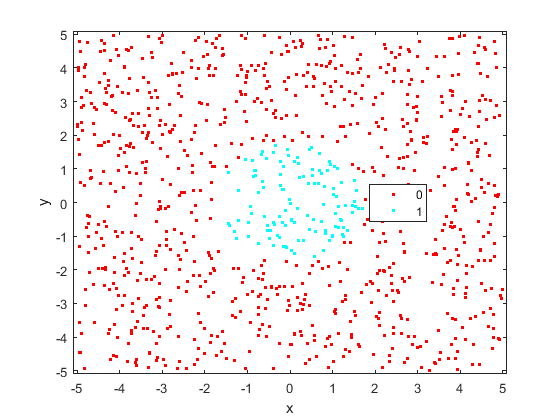
\includegraphics[width=5cm, height=5cm]{figures/scatter.png}
	\caption{Diese Grafik zeigt...}
\end{figure}

Lorem ipsum dolor sit amet, consetetur sadipscing elitr, sed diam nonumy eirmod tempor invidunt ut labore et dolore magna aliquyam erat, sed diam voluptua. At vero eos et accusam et justo duo dolores et ea rebum. Stet clita kasd gubergren, no sea takimata sanctus est Lorem ipsum dolor sit amet. Lorem ipsum dolor sit amet, consetetur sadipscing elitr, sed diam nonumy eirmod tempor invidunt ut labore et dolore magna aliquyam erat, sed diam voluptua. At vero eos et accusam et justo duo dolores et ea rebum. Stet clita kasd gubergren, no sea takimata sanctus est Lorem ipsum dolor sit amet (nach \cite{Russell.2018}).


\newpage








\section{Schluss}

Lorem ipsum dolor sit amet, consetetur sadipscing elitr, sed diam nonumy eirmod tempor invidunt ut labore et dolore magna aliquyam erat, sed diam voluptua. At vero eos et accusam et justo duo dolores et ea rebum. Stet clita kasd gubergren, no sea takimata sanctus est Lorem ipsum dolor sit amet.

\begin{table}[h]
	% Für eine zentrierte Tabelle "\centering" hinzufügen
	\centering
	\begin{tabular}{|c|c|c|} \hline
		Spalte 1 & Spalte 2 & Spalte 3 \\ \hline \hline
		B & C & D \\ \hline
		X & Y & Z \\ \hline
	\end{tabular}
	\caption{Tabelle}
\end{table}




\newpage

%%%%%%%%%%%%%%%%%%%%%%%%%%%%%%%%%% Abbildungsverzeichnis %%%%%%%%%%%%%%%%%%%%%%%%%%%%%%%%%%%%%

\pagestyle{plain}
\addcontentsline{toc}{section}{Abbildungsverzeichnis}
\listoffigures







%%%%%%%%%%%%%%%%%%%%%%%%%%%%%%%%% Literaturverzeichnis %%%%%%%%%%%%%%%%%%%%%%%%%%%%%%%%%%%%%%%

\newpage

% Wird das Literaturverzeichnis nicht angezeigt, muss in den Optionen - TeXstudio konfigurieren - Erzeugen - Standard Bibliographieprogramm auf "Biber" umgestellt werden.
\printbibliography[heading=bibintoc,title={Literaturverzeichnis}]
\pagestyle{plain}

\newpage

\section*{Erklärung}

Ich versichere wahrheitsgemäß, die Arbeit selbstständig verfasst, alle benutzten Hilfsmittel vollständig und genau angegeben und alles kenntlich gemacht zu haben, was aus Arbeiten anderer unverändert oder mit Abänderungen entnommen wurde sowie die Satzung des KIT zur Sicherung guter wissenschaftlicher Praxis in der jeweils gültigen Fassung beachtet zu haben.

\vspace{3cm}

\hspace{0.5cm} Karlsruhe, den \today



\end{document}